\documentclass[a4paper, 11pt]{article}
\usepackage[polish]{babel}
\usepackage[MeX]{polski}
\usepackage[utf8]{inputenc}
\usepackage[T1]{fontenc}
\usepackage{latexsym}
%\usepackage{times}
\usepackage{graphicx,wrapfig}
%\usepackage{anysize}
%\usepackage{tikz}
%\usetikzlibrary{calc,through,backgrounds,positioning}
\usepackage{anysize}
\usepackage{float}
%\usepackage{stmaryrd}
%\usepackage{amssymb}
%\usepackage{amsthm}
%\marginsize{3cm}{3cm}{3cm}{3cm}
%\usepackage{amsmath}
%\usepackage{color}
%\usepackage{listings}
%\usepackage{enumerate}
%\lstloadlanguages{Ada,C++}

		\newcommand\tab[1][1cm]{\hspace*{#1}}

\begin{document}	
	% \noindent -  w tym akapicie nie bedzie wciecia
	% \ indent - to jest aut., ale powoduje ze jest wciecie
	% \begin{flushleft}, flushright, center - wyrownianie akapitu
	% \textbf{pogrubiany tekst}
	% \textit{kursywa} 
	% 					STRONY 
	%  http://www.codecogs.com/latex/eqneditor.php 
	%  http://www.matematyka.pl/latex.htm
	% 
	
	\begin{titlepage}
		
		
		\newcommand{\HRule}{\rule{\linewidth}{0.5mm}} % Defines a new command for the horizontal lines, change thickness here
		
		\center % Center everything on the page
		
		%----------------------------------------------------------------------------------------
		%	HEADING SECTIONS
		%----------------------------------------------------------------------------------------
		
		\textsc{\LARGE Akademia Górniczo-Hutnicza im. Stanisława Staszica}\\[1.5cm] % Name of your university/college
		\textsc{\Large Kraków}\\[0.5cm] % Major heading such as course name
		\textsc{\large }\\[0.5cm] % Minor heading such as course title
		
		%----------------------------------------------------------------------------------------
		%	TITLE SECTION
		%----------------------------------------------------------------------------------------
		
		\HRule \\[0.4cm]
		{\fontsize{38}{50}\selectfont Generator specyfikacji logicznej}
		%	{ \Huge \bfseries} Symulator pożaru lasu\\[0.3cm] % Title of your document
		\HRule \\[5.5cm]
		
		%----------------------------------------------------------------------------------------
		%	AUTHOR SECTION
		%----------------------------------------------------------------------------------------
	
\begin{minipage}{0.4\textwidth}
\begin{flushleft} \large 
\emph{Autorzy:}\\
Marcin \textsc{Jędrzejczyk}\\ % Your name
Paweł \textsc{Ogorzały} \\

\end{flushleft}
\end{minipage}
~
\begin{minipage}{0.4\textwidth}
\begin{flushright} \large
\emph{Prowadzący:}\\
 Dr inż. Radosław \textsc{Klimek}  % Supervisor's Name
\end{flushright}
\end{minipage} \\[5cm]
		
		
		%----------------------------------------------------------------------------------------
		%	DATE SECTION
		%----------------------------------------------------------------------------------------
		
		{\large \today}\\[3cm] % Date, change the \today to a set date if you want to be precise
		
		%----------------------------------------------------------------------------------------
		%	LOGO SECTION
		%----------------------------------------------------------------------------------------
		
		%\includegraphics{Logo}\\[1cm] % Include a department/university logo - this will require the graphicx package
		
		%----------------------------------------------------------------------------------------
		
		\vfill % Fill the rest of the page with whitespace
		
	\end{titlepage}
	

	
	%\tableofcontents
	\vfill
	\newpage
	%\pagebreak
	
	
	
	%\setlength{\parskip}{1ex plus 0.5ex minus 0.2ex}
	
%	\section{Wstęp}
    %	
	
	\indent
	\section{Cel projektu}
	%w sumie opisać co mamy zrobić	
	Celem projektu jest wytworzenie programu, który dla podanego diagramu będzie w stanie go sparsować do formatu pozwalającego na wygenerowanie specyfikacji logicznej.
	
	\section{Powód tworzenia generatora}
	%Klimek sam wyisał czemu, musimy to tu wstawić
	\begin{itemize}
	\item Ręczne tworzenie specyfikacji logiki jest trudne dla niedoświadczonych w tym użytkowników.
	\item Formalna weryfikacja modelu oprogramowania pozwala obniżyć koszty i zwiększyć niezawodność.
	\item Brak takich narzędzi.
	\end{itemize}
	\section{Ważne}
	\begin{itemize}
	\item Diagram aktywności musi składać się z wcześniej zdefiniowanych wzorców, zagnieżdżanie jest dozwolone.
	\item Diagram aktywności składa się tylko z atomicznych aktywności, zidentyfikowanych podczas tworzenia scenariuszy przypadków użycia.
	\item Generator musi działać automatycznie, usuwa to błąd ludzki.
	\end{itemize}
	\section{Specyfikacja logiczna}
	
	Automatyzacja generowania specyfikacji logicznej, rozumianej jako zestawu temporalnych formuł logicznych jest kluczowym zagadnieniem. Opiera się ono na kilku założeniach:
	\begin{itemize}
	\item Modele oprogramowania są opracowane jako przepływy pracy. Przepływ to postępujące zdarzenie, zadanie, interakcja obejmujące proces pracy.
	\item Przepływy pracy są opracowany przy użyciu zdefiniowanych wzorców.
	\item Każdy wzorzec przepływu pracy jest powiązany z zdefiniowanymi wcześniej formułami logicznymi opisującymi własności tego wzorca.
	\end{itemize} 
	Elementarny zestaw formuł oznaczony \textit{elem($a_1,...,a_n)$} lub po prostu \textit{elem()}, nad atomowymi formułami $a_1,...,a_n$, gdzie formuła atomowa jest podzielona na trzy podzbiory parami rozłączne:
	\begin{itemize}
		\item Pierwsze podzbiór, który zawiera co najmniej jeden element to \textit{argumenty wejściowe}
		\item Drugi podzbiór, który może być pusty to \textit{zwykłe argumenty}
		\item Trzeci podzbiór, który zawiera co najmniej jeden element to \textit{argumenty wyjściowe}
	\end{itemize}
	jest zbiorem formuł \textit{$f_1,...f_m$} składniowo poprawnych oraz $f_1,...,f_m$ gdzie $m>0$ są temporalnymi formułami logicznymi to
	\textit{$elem()=\{f_1,...,f_m\}.$}
	\\
	\\
	Wprowadźmy pojęcie formuły wejścia/wyjścia należących do klasycznej logiki. $f_{en}$ i $f_{ex}$ opisują logiczne okoliczności związane z otwarciem i zamknięciem wzorca. $f_{en}$ jest spełnione, gdy pewne początkowe działania są aktywne. Na przykład $a\wedge b$ dla $f_{en}$ oznacza, że gdy wykonanie wzorca jest zainicjowane, obie aktywności \textit{a} i \textit{b} są spełnione. $a\vee b$ dla $f_{ex}$ oznacza, że gdy wykonywanie wzorca ma zostać zakończone wtedy działania \textit{a} oraz \textit{b} są aktywne. Podsumowując $f_{en}$ oraz $f_{ex}$ opisują odpowiednio pierwsze i ostatnie aktywne działania wzorca.
	\\
	\\
	Wzór zestawu formuł oznaczony \textit{$pat(a_1,...,a_n)$} lub uproszczając \textit{$pat()$}, nad formułami atomicznymi $a_1,...,a_n$ jest zbiorem $pat(a_1,...,a_n) \equiv \{f_{en},f_{ex}\} \cup elem(a_1,...,a_n)$ a jej elementy są częściowo uporządkowane w taki sposób, że $f_{en}$ jest zawsze pierwszym elementem, $f_{ex}$ jest zawsze drugim elementem.
	\\
	Dla każdego wzorca \textit{pat}, $pat.f_{en}$ i $pat.f_{ex}$ oznacza odpowiednio wejściowe i wyjściowe formuły wzorca.
	\\
	\\
	Wyrażenie logiczne $W_L$ jest strukturą stworzoną na podstawie następujących reguł:
	\begin{itemize}
		\item każdy elementarny zestaw $pat(a_i)$, gdzie $i>0$ i każde $a_i$ jest formułą atomiczną, jest wyrażeniem logicznym
		\item każde $pat(A_i)$, gdzie $i>0$ i każde $A_i$ jest
		\begin{itemize}
			\item formułą atomiczną, lub
			\item wyrażeniem logicznym \textit{pat()}
		\end{itemize}
		jest także wyrażeniem logicznym
	\end{itemize}
	Wyrażenie logiczne stworzone w powyższy sposób jest dobrze sformatowane. Prostym przykładem wyrażenia logicznego jest $w=Seq(Split(a,b,c),Cond(d,e,f))$ znaczenie wszystkich wzorców jest intuicyjne i nie jest formalnie zdefiniowane. $|w|$ oznacza długość wyrażenia logicznego, które jest liczbą wzorców w wyrażeniu. $w[i]$ oznacza wzór na i-tej pozycji w wyrażeniu logicznym $w$, np. $w[2]=Split$. $|w[i]|$ oznacza liczbę argumentów i-tego wzoru, np. $|w[1]|=2$ a $|w[3]|=3.$
	\\
	\\
	Zestaw \textit{predefiniowanych wzorców $\Pi$} jest to zestaw, który zawiera wszystkie dopuszczalne wzorce przepływu dla procesu rozwoju branego pod uwagę. Zbiór \textit{wzorców własności P}, lub w skrócie \textit{własności P} to zestaw logicznych atrybutów i cechy, które wzorce wymienione w \textit{$\Pi$} posiadają.
	\textit{"'"} to selektor odpowiedniego obiektu wzorca, np. \textit{$w[i]'P$} oznacza własność \textit{P}, która zawiera formuły dla wzorca na i-tej pozycji w wyrażeniu \textit{w}. \textit{"."} jest selektorem formuły w elementarnym zbiorze, do którego odnosi się wzorzec w wyrażeniu logicznym, np. $w[i]'P.f_{en}$ oznacza formułę $f_{en}$ w elementarnym zbiorze i-tego wzorca w wyrażeniu. $"\uparrow"$ jest selektorem argumentów w wzorcu. $w[i]\uparrow a_j$ oznacza argument $a_j$ i-tego wzorca w wyrażeniu logicznym \textit{w}.
	\\
	\\
	Niech $w^c$ dla wyrażenia logicznego \textit{w} będzie zagregowaną formułą wejściową (wyjściową), gdzie agregowana formuła jest wyliczana na podstawie następujących reguł:
	\begin{itemize}
		\item jeśli nie ma wzorca w miejscu jakiejkolwiek formuły atomicznej/argumentu, która składniowo należy do formuły $f_{en}$ (lub $f_{ex}$) \textit{w}, wtedy $w^e$ jest równe $f_{en}$ ($w^x$ jest równe $f_{ex}$).
		\item jeśli istnieje wzorzec, powiedzmy $t()$ w miejscu jakiegokolwiek atomicznego argumentu powiedzmy \textit{r}, który składniowo należy do formuły $f_{en}$ (lub $f_{ex}$) \textit{w}, wtedy \textit{r} jest zastępowane przez $t^e$ (lub $t^x$) dla każdego przypadku.
	\end{itemize}
	\textbf{Algorytm - Generowanie specyfikacji logicznej ($A$)}\\
	\textbf{Input:} Wyrażenie logiczne $W_L$, zdefiniowane wzorce przepływu(nie puste) $P$\\
	\textbf{Output:} Specyfikacja logiczna $L$
	
	$L:=0$
	
	\textbf{for} $i:=1$ \textbf{to} $|W_L|$ \textbf{do}\\
	\tab $L2:=W_L[i]P'\backslash \{W_L[i]'P.f_{en},W_L[i]'P.f_{ex}\};$\\	
	\tab \textbf{for} $j:=1$ \textbf{to} $|W_L[i]|$ \textbf{do}\\
	\tab \tab \textbf{if} $W_L[i] \uparrow a_j$ is non-atomic then \\
	\tab \tab \tab	$agg:=(W_L[i]'P\uparrow a_J())^e+"V"+(W_L[i]'P\uparrow a_J())^x;$\\
	\tab \tab \tab	replace in L2 every pattern $W_L[i]'P\uparrow a_j()$ by agg;\\
	\tab \tab	\textbf{end if}\\
	\tab  \textbf{end for}\\
	\tab  L:=L $\cup$ L2 \\
	\tab[0.5cm]\textbf{end for}
	\\
	\\
	Specyfikacja logiczna \textit{L} składa się ze wszystkich wzorców uzyskanych z wyrażenia logicznego $W_L$ przy stałych właściwościach \textit{P} 
	\\
	$L(W_L,P)=\{f:f\in A(W_L,P)\}$
	\section{Algorytmy}
	
	Wzorce przepływu:
	\begin{itemize}
	\item Sekwencja, sequence
	\item Współbieżność, concurrent fork/join
	\item Pętla while, loop while
	\item Rozgałęzienie, branching
	\end{itemize}
	\begin{figure}[H]
		\centerline{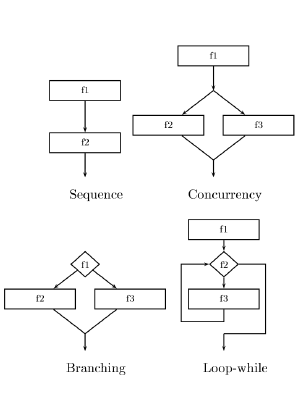
\includegraphics[scale=1.5]{workflows}}
		\caption{Wzorce przepływu}
	\end{figure}%
		
	\noindent Wyrażenie logiczne $W_L$ jest strukturą stworzoną według poniższych zasad:\\
	\begin{itemize}
	\item każdy elementarny zbiór $pat(a_i)$, gdzie $i>0$ i każde $a_i$ jest formułą atomiczną, jest wyrażeniem logicznym,
	\item każde $pat(A)$, gdzie $i>0$ i każde $A_i$ jest albo
	\begin{itemize}
	\item atomiczną formułą lub
	\item logicznym wyrażeniem $pat()$
	\end{itemize}
	także jest wyrażeniem logicznym.
	\end{itemize}
	\noindent Wstępny algorytm:
	\begin{enumerate}
	\item Analiza diagramów aktywności w celu wyciągnięcia z nich wcześniej zdefiniowanych wzorców przepływu.
	\item Przetłumaczenie wyłuskanych wzorców na wyrażenia logiczne $ W_L$.
	\item Generowanie specyfikacji logicznej $L$ z wyrażeń logicznych, %i.e. receiving a set of temporal logics formulas.
	\end{enumerate}
	
 		\noindent Algorytm $\Pi$ generujący specyfikację logiczną :\\
		\begin{enumerate}
		\item Na początku specyfikacja jest pusta, np. L={\o};
		\item Najbardziej zagnieżdżone wzorce są przetwarzane jako pierwsze, a następnie mniej zagnieżdżone;
		\item Jeśli obecnie analizowany wzorzec składa się wyłącznie z formuł atomicznych, specyfikacja logiczna jest rozszerzana, poprzez sumowanie zbiorów, których formuły są złączone z obecnie analizowanym wzorcem pat(), np. $L=L \cup pat() $;
		\item Jeżeli jakiś argument jest wzorem sam w sobie to:
		\begin{itemize}
		\item po pierwsze formuła $f1$  , a potem
		\item formuła $fk$
		\end{itemize}
		tego wzoru(jeśli jakiegoś), lub w innym wypadku wziąć pod uwagę tylko najbardziej zagnieżdżony daleko? na lewo lub prawo,odpowiednio, są podstawiane osobno w miejsce wzorca jako argument.
		\end{enumerate}


	\section{Przykłady}
Podane wzorce P:
	\begin{itemize}
					\item Sequence(f1,f4)
		\begin{itemize}
			\item f1 $ \Rightarrow $  $\diamond$f4 	
			\item $\neg$f1 $ \Rightarrow $ $\neg$ $\diamond$f4
			\item $\Box$ $\neg$( f1  $\wedge$  f4 )
		\end{itemize}
		\item Concurrency(f1,f2,f3,f4)
		\begin{itemize}
			\item f1 $ \Rightarrow $  $\diamond$f2  $\wedge$  $\diamond$f3
			\item $\neg$f1 $ \Rightarrow $  $\neg$( $\diamond$f2  $\wedge$  $\diamond$f3)
			\item f2  $\wedge$  f3  $ \Rightarrow$  $\diamond$f4
			\item $\neg$(f2  $\wedge$  f3)  $ \Rightarrow $  $\neg$ $\diamond$f4
			\item $\Box$ $\neg$(f1  $\wedge$  (f2 \ $\vee$  f3))
			\item $\Box$ $\neg$((f2 \ $\vee$  f3)  $\wedge$  f4)
			\item $\Box$ $\neg$(f1  $\wedge$  f4)	
		\end{itemize}
		\item Branching(f1,f2,f3,f4)
		\begin{itemize}
			\item f1  $ \Rightarrow $  ($\diamond$f2  $\wedge$  $\neg$ $\diamond$f3)  $\vee$  ($\neg$ $\diamond$f2  $\wedge$  $\diamond$f3)
			\item $\neg$f1  $ \Rightarrow $  $\neg$(($\diamond$f2  $\wedge$  $\neg$ $\diamond$f3) \ $\vee$  ($\neg$ $\diamond$f2  $\wedge$  $\diamond$f3))
			\item f2 $\vee$  f3  $ \Rightarrow $  $\diamond$f4
			\item $\neg$(f2 \ $\vee$  f3)  $ \Rightarrow$  $\neg$ $\diamond$f4
			\item $\Box$ $\neg$(f1  $\wedge$  f4)
			\item $\Box$ $\neg$(f2  $\wedge$  f3)
			\item $\Box$ $\neg$(f1  $\wedge$  (f2 \ $\vee$  f3))
			\item $\Box$ $\neg$((f2 \ $\vee$  f3)  $\wedge$  f4)
		\end{itemize}
		\item LoopWhile(a,b,c,d)
		\begin{itemize}
			\item f1$\Rightarrow$ $\diamond$f2
			\item $\neg$f1$\Rightarrow$ $\neg$ $\diamond$f2
			\item f2  $\wedge$  c(f2) $\Rightarrow$ $\diamond$c $\wedge$  $\neg$ $\diamond$f4
			\item $\neg$(f2  $\wedge$  c(f2)) $\Rightarrow$ $\neg$($\diamond$f3 $\wedge$  $\neg$ $\diamond$f4)
			\item f2  $\wedge$  $\neg$c(f2) $\Rightarrow$ $\neg$ $\diamond$f3  $\wedge$  $\diamond$f4
			\item $\neg$(f2  $\wedge$  $\neg$c(f2) $\Rightarrow$ $\neg$($\neg$ $\diamond$f3 $\wedge$  $\diamond$f4)
			\item f3 $\Rightarrow$ $\diamond$f2
			\item $\neg$f3$\Rightarrow$ $\neg$ $\diamond$f2
			\item $\Box$ $\neg$(f1  $\wedge$  f2)
			\item $\Box$ $\neg$(f1  $\wedge$  f3)
			\item $\Box$ $\neg$(f1  $\wedge$  f4)
			\item $\Box$ $\neg$(f2  $\wedge$  f3)
			\item $\Box$ $\neg$(f2  $\wedge$  f4)
			\item $\Box$ $\neg$(f3  $\wedge$  f4) 
		\end{itemize}
	\end{itemize}	
	
	Wyjście programu dla:
	TUTAJ OBRAZEK UML, POTEM WYCIĄGNIĘTA FORMUŁA I WYNIK
	\begin{itemize}
	\item $W_L= $ Concur(a,b,c,d) to:\\
	$L= \{ a   \Rightarrow     \diamond b   \wedge    \diamond c $,
		$	  \neg a   \Rightarrow     \neg (  \diamond b   \wedge    \diamond c)$,
			$ b   \wedge   c    \Rightarrow    \diamond d$,
			$  \neg (b   \wedge   c)    \Rightarrow     \neg   \diamond d$,
			$  \Box   \neg (a   \wedge   (b \  \vee   c))$,
			$  \Box   \neg ((b \  \vee   c)   \wedge   d)$,
			$  \Box   \neg (a   \wedge   d)\}$
	
	\item 	$W_L=$ Seq(Seq(a,b),c) to: \\
	$ L=\{  a \Rightarrow \diamond b , \neg a\Rightarrow \neg \diamond b, \Box \neg (a \wedge  b)\} \cup $ \\
	$ \cup \{ a \Rightarrow c , \neg a\Rightarrow \neg \diamond c, \Box\neg (a \wedge  c)\} \cup $\\
	$ \cup \{ b \Rightarrow c , \neg b\Rightarrow \neg \diamond c, \Box \neg (b \wedge  c)\} $
	
	\item Branch(Seq(a,b),c,d,e) to:\\
	$ L=$\\$ \{  a \Rightarrow \diamond b , \neg a\Rightarrow \neg \diamond b, \Box \neg (a \wedge  b)\} $ 
	$\cup 	\{	  a    \Rightarrow    ( \diamond c   \wedge    \neg   \diamond d)   \vee   ( \neg   \diamond c   \wedge    \diamond d)$,
			  $ \neg a    \Rightarrow     \neg (( \diamond c   \wedge    \neg   \diamond d)  \vee  \vee ( \neg   \diamond c   \wedge    \diamond d))$,
			 $ c  \vee d    \Rightarrow     \diamond e $,
			  $ \neg (c  \vee   d)    \Rightarrow    \neg   \diamond e$ ,
			   $\Box   \neg (a   \wedge   e)$ ,
			   $\Box   \neg (c   \wedge   d)$,
			   $\Box   \neg (a   \wedge   (c \  \vee   d))$,
			   $\Box   \neg ((c \  \vee   d)   \wedge   e)\} $			  
	$\cup 	\{	  b    \Rightarrow    ( \diamond c   \wedge    \neg   \diamond d)   \vee   ( \neg   \diamond c   \wedge    \diamond d)$,
			  $ \neg b    \Rightarrow     \neg (( \diamond c   \wedge    \neg   \diamond d) \  \vee   ( \neg   \diamond c   \wedge    \diamond d))$,
			 $ c  \vee   d    \Rightarrow     \diamond e $,
			  $ \neg (c \  \vee   d)    \Rightarrow    \neg   \diamond e$ ,
			   $\Box   \neg (b   \wedge   e)$ ,
			   $\Box   \neg (c   \wedge   d)$,
			   $\Box   \neg (b   \wedge   (c   \vee   d))$,
			   $\Box   \neg ((c \  \vee   d)   \wedge   e)\}$
			 		   		
	\end{itemize}
	\section{Struktura programu}
	\begin{figure}[H]
		\centerline{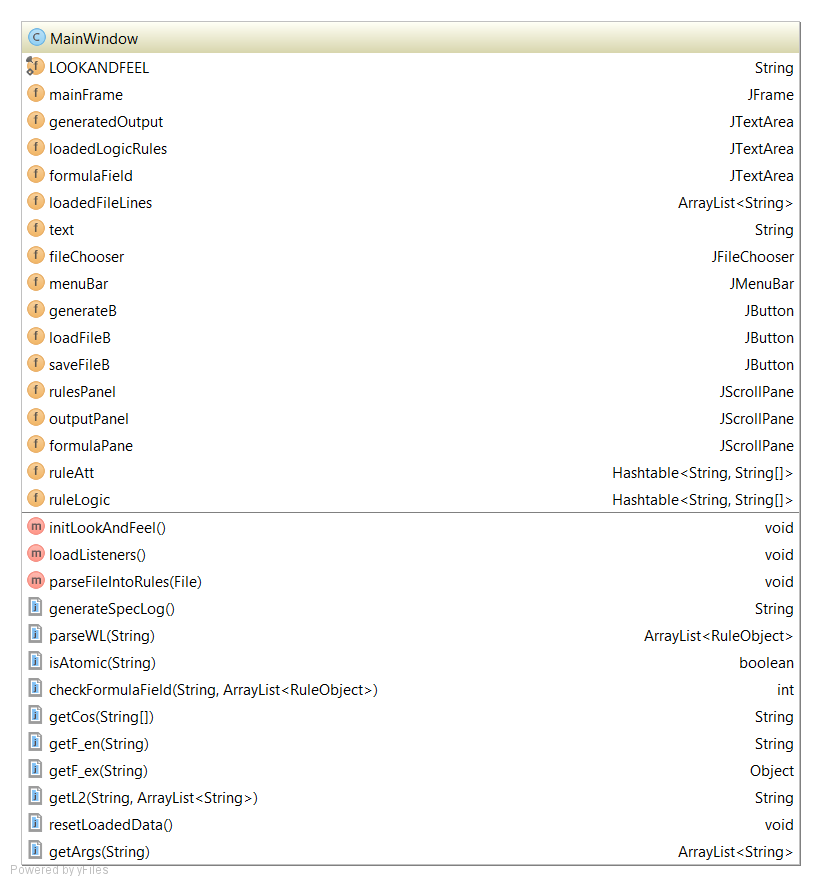
\includegraphics[scale=0.6]{diagram}}

	\end{figure}%
	\begin{figure}[H]
		\centerline{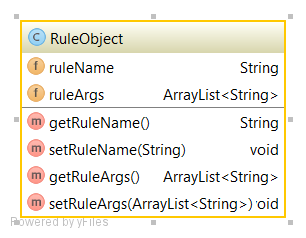
\includegraphics[scale=0.6]{diagram2}}

	\end{figure}%
	\section{Wygląd GUI}
	
	\begin{figure}[H]
	\centerline{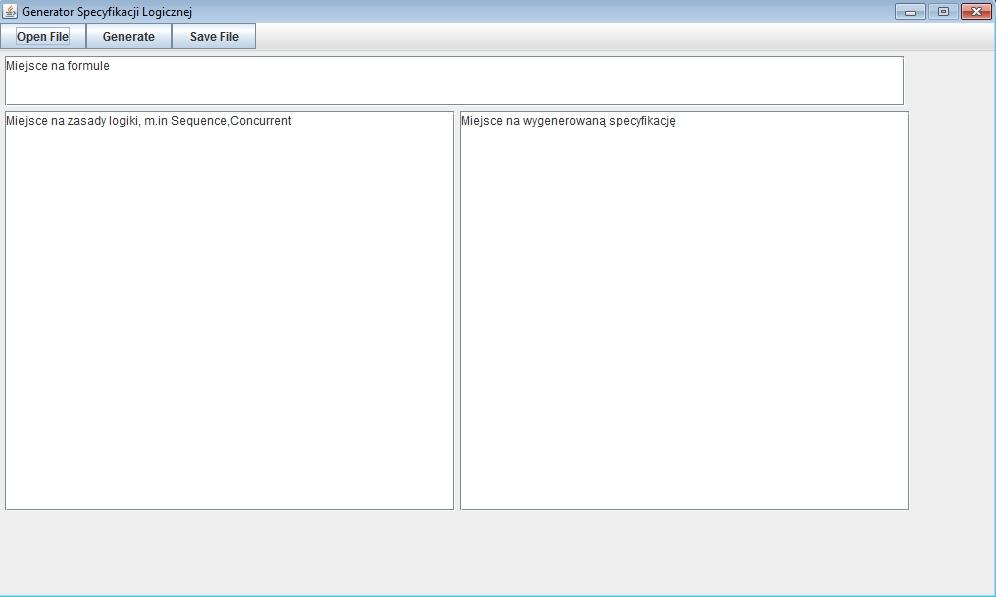
\includegraphics[scale=0.6]{GUI}}
	\caption{Interfejs graficzny}
	\end{figure}%
	
	WCZYTYWANIE ZASAD LOGIKI	
	
	OPCJA ZAPISU-OBRAZEK
	
	GENEROWANIE
	
	
	

	
	\section{Literatura}
	%\indent	
	\textbf{Radosław Klimek:} From Extraction of Logical Specifications to Deduction-Based Formal Verification of Requitements Models. Strony 61-75.\\
		\textbf{Radosław Klimek:} Elicitation of logical specifications from RUP-like processes for formal verification.\\
	
	
	
\end{document}
